\documentclass[a4paper,11pt]{report}

% General tools
\usepackage{etoolbox}

\usepackage[utf8]{inputenc}

% Fonts
\usepackage[T1]{fontenc}

% Monospace
\usepackage{sourcecodepro}

% Bibtex and biblatex for references
\usepackage[backend=biber,
    style=chem-angew,
    sortlocale=en_GB,
    natbib=true,
    url=false,
    doi=true,
    eprint=false
]{biblatex}
\addbibresource{biblatex-res.bib}

% Glossary
\usepackage[xindy,toc]{glossaries}

% Language
\usepackage[english]{babel}
\usepackage{blindtext}

% Page style
\usepackage{fullpage} % page margins to 1.5cm
\usepackage{fancyhdr} % headers and footers

% Colors & graphics
\usepackage[table]{xcolor}    % colors
\usepackage[pdftex]{graphicx} % graphics importing
\usepackage[pdf]{graphviz}
\usepackage{auto-pst-pdf}

% Misc
\usepackage{titlesec} % section titles formatting
\usepackage{minted}   % code highlighting
\usepackage{lscape}   % landscape
\usepackage{tikz}     % charts in LaTeX
\usepackage{amsmath}  % better math
\usepackage{amsfonts}
\usepackage{amssymb}
\usepackage{float}    % floats
\usepackage[small,justification=centering]{caption}
\usepackage{microtype} % typographic improvements

\usepackage[shortlabels]{enumitem}

% Appendix
\usepackage[toc,page]{appendix}

% UML
\usepackage{extra-package/tikz-uml}

% Paragraphs
\usepackage{parskip}
\usepackage[defaultlines=3,all]{nowidow}

\usepackage[autostyle]{csquotes}

% Chapter titles
% Remove space before title
\titlespacing{\chapter}{0pt}{*-4}{*3}
% Remove "Chapter N" and use a sans-serif font
\titleformat{\chapter}[hang]{\bf\huge}{\thechapter}{1pc}{}
% Change chapter page style
\patchcmd{\chapter}{plain}{fancy}{}{}

% Tables
\usepackage{multirow}

% Cross-references
\usepackage{hyperref}

% Metadata
% --------
% ==============================
% Authors of the LaTeX template:
%   - Sylvain Julmy
%   - Marc Demierre
% ==============================

% Metadata for this report
% ------------------------
\newcommand{\School}{University of Applied Sciences Western Switzerland}
\newcommand{\Faculty}{MSE - Software Engineering}
\newcommand{\Place}{Fribourg}

% Course
\newcommand{\Course}{Deepening project}
\newcommand{\Title}{KlugHDL : a SpinalHDL diagram generator}

% Supervisors (professors)
\newcommand{\Supervisors}{Mudry Pierre-André}

% Students
\newcommand{\Authors}{Julmy Sylvain}



% Header and footer
% -----------------
\pagestyle{fancy}
\lhead[]{\Course}
\chead[]{}
\rhead[]{\Place, \today}

\setlength{\headheight}{14pt}
\setlength{\headsep}{14pt}

\newcommand{\HRule}{\rule{\linewidth}{0.5mm}}

\newcommand{\BlackLine}{\noindent\rule[0.5ex]{\linewidth}{1pt}\\}

% Java
\newminted{java}{frame=single, framesep=6pt, breaklines=true, fontsize=\scriptsize}
\newmintedfile{java}{frame=single, framesep=6pt, breaklines=true, fontsize=\scriptsize}

% Scala
\newminted{scala}{frame=single, framesep=6pt, breaklines=true, fontsize=\scriptsize}
\newmintedfile{scala}{frame=single, framesep=6pt, breaklines=true, fontsize=\scriptsize}

% Python
\newminted{python}{frame=single, framesep=6pt, breaklines=true, fontsize=\scriptsize}
\newmintedfile{python}{frame=single, framesep=6pt, breaklines=true, fontsize=\scriptsize}

% Plain text
\newminted{text}{frame=single, framesep=6pt, breaklines=true, breakanywhere, fontsize=\scriptsize}
\newmintedfile{text}{frame=single, framesep=6pt, breaklines=true, breakanywhere, fontsize=\scriptsize}

% VHDL
\newminted{vhdl}{frame=single,framesep=6pt, breaklines=true, fontsize=\scriptsize}
\newmintedfile{vhdl}{frame=single, framesep=6pt, breaklines=true, fontsize=\scriptsize}

% JavaScript
\newminted{js}{frame=single,framesep=6pt, breaklines=true, fontsize=\scriptsize}
\newmintedfile{js}{frame=single, framesep=6pt, breaklines=true, fontsize=\scriptsize}


% Document
% --------
\begin{document}

\begin{titlepage}
    \begin{center}

        % only works if a paragraph has started.
        
\includegraphics[width=0.8\textwidth]{img/mse_logo}~\\[1.5cm]
        \textsc{\Large \School}\\[0.25cm]
        \textsc{\Large \Faculty}\\[1.5cm]
        \textsc{\LARGE \Course}\\[0.5cm]

        % Title
        \HRule \\[0.4cm]
        { \huge \bfseries \Title\\[0.4cm] }
        \HRule \\[1.5cm]

        % Author and supervisor
        \begin{minipage}[t]{0.4\textwidth}
            \begin{flushleft} \Large
                \emph{Author:}\\ \Authors
            \end{flushleft}
        \end{minipage}
        \begin{minipage}[t]{0.4\textwidth}
            \begin{flushright} \Large
                \emph{Supervisor:}\\\Supervisors
            \end{flushright}
        \end{minipage}~\\[1.5cm]

        \begin{center}
            
\includegraphics[scale=0.7]{img/logo_hes-so}
        \end{center}

        \vfill

        % Bottom of the page
        {\large \Place, \today}

    \end{center}
\end{titlepage}

% Uncomment this for a table of contents

\tableofcontents

\chapter{Introduction} %{{{
\label{cha:Introduction}

A program is a sequence of mathematical instruction which are written by a human and executed by a computer.
The VHDL langage has been created to describe digital and signals systems such as field-programmable gate arrays
and integrated circuits\cite{wiki-vhdl}.The problem is that VHDL is an old, verbose and tricky language.

SpinalHDL has been created to fight thos disadvantage. The main goal of a DSL (Domain Specific Langage) is to offer a more plaisant way to code and that's what dose SpinalHDL. Has written before, the code is written by a human and by using SpinalHDL, the human became happier than using just the VHDL.

KlugHDL is an another tools to make the human happiest, it's a component diagram generator which offer some

\section{Context} %{{{
\label{sec:Context}

SpinalHDL is a programming language to describe digital hardware and generate the corresponding in VHDL (or Verilog). SpinalHDL is written in Scala as a DSL and has multiple advantages\cite{github-spinalhdl} :
\begin{itemize}
    \item No restriction to the genericity of your hardware description by using Scala constructs
    \item No more endless wiring. Create and connect complex buses like AXI in one line.
    \item Evolving capabilities. Create your own buses definition and abstraction layer.
    \item Reduce code size by a high factor, especially for wiring. Allowing you to have a better visibility, more productivity and fewer headaches.
    \item Free and user friendly IDE. Thanks to scala world for auto-completion, error highlight, navigation shortcut and many others
    \item Extract information from your digital design and then generate files that contain information about some latency and addresses
    \item Bidirectional translation between any data type and bits. Useful to load a complex data structure from a CPU interface.
    \item Check for you that there is no combinational loop / latch
    \item Check that there is no unintentional cross clock domain 
\end{itemize}

The code \ref{lst:spinalhdl_example_and_gate} shows a AND gate written with SpinalHDL with the corresponding generated VHDL code, we could see the similarity between the two code.

\begin{listing}[h] % {{{
    \centering
    
    \begin{minipage}[c]{0.45\textwidth}
    \begin{scalacode}
    import spinal.core._

    class AND extends Component
    {
        val io = new Bundle
        {
            val a = in Bool
            val b = in Bool
            val c = out Bool
        }

        io.c := io.a & io.b
    }    
    \end{scalacode}
    \end{minipage}
    \hfill
    \begin{minipage}[c]{0.45\textwidth}
    \begin{vhdlcode}
    entity AND_1 is
        port( 
            io_a : in std_logic;
            io_b : in std_logic;
            io_c : out std_logic 
        );
    end AND_1;

    architecture arch of AND_1 is

    begin
      io_c <= (io_a and io_b);
    end arch;
    \end{vhdlcode}
    \end{minipage}
    \caption{Example of a AND gate written in SpinalHDL and the corresponding generated VHDL code}
    \label{lst:spinalhdl_example_and_gate}
\end{listing} %}}}

%}}} section Context

\section{Goal} %{{{
\label{sec:Goal}

The goal of the project is to produce an application which is analysing a spinalhdl program in order to produce a block diagramm of the corresponding hardware description. This application should offer the following activities :

\begin{itemize}
    \item Display the complete graph of the programm
    \item Navigate through all the hierarchical level of the programm (Component inside another component)
    \item The edges should display some information about the signals :
    \begin{itemize}
        \item type
        \item input or output
        \item ...
    \end{itemize}
    \item A Hierarchical view (like in filesystems or in Quartus)
    \item A filter functionnality in order to view only some specific component
\end{itemize}

The application is going to be develop, firstable, in a standalone version and next could be develop into a plugin version for Eclipse or IntelliJ.

%}}} section Goal

\section{Document overview} %{{{
\label{sec:Document overview}

TODO

%}}} section Document overview

%}}} chapter Introduction 

\chapter{Analysis}
\label{cha:Analysis}

In this chapter, we would discuss about the "What do we want ?" questions. It
means what need the final product based on the goal of the project. The other
part is about the actual state of SpinalHDL. We are not presenting all the
implementation or conception, just a small part is useful for this
project. Finally, we introduce the concept of the SpinalHDL's component and AST
(Abstract Syntax Tree).

\section{What do we want ?}
\label{sec:What do we want ?}

Based on the goal of the project at section \ref{sec:Goal}, we expose what the
end user of SpinalHDL want to do with KlugHDL. The figure
\ref{fig:use_case_klughdl} show the use case of KlugHDL.

\begin{figure}[H]
    \centering

    \begin{tikzpicture}

        \umlactor[x=0,y=3,name=user]{SpinalHDL user}
        \umlactor[x=0,y=0,name=spinal]{SpinalHDL}

        \begin{umlsystem}[x=3,y=0]{KlugHDL}
            \umlusecase[x=4,y=6,name=UCA,width=180]{Generate a component diagram}
            \umlusecase[x=4,y=4.9,name=UCB,width=180]{View a component diagram}
            \umlusecase[x=4,y=3.7,name=UCC,width=180]{Display, hide and toggle
              the hierarchical tree view of the programm}
            \umlusecase[x=4,y=2.6,name=UCD,width=180]{Filter the hierarchical view}
            \umlusecase[x=4,y=1.5,name=UCE,width=180]{Enter a component}
            \umlusecase[x=4,y=0.4,name=UCF,width=180]{Go out of a component}
            \umlusecase[x=4,y=-0.8,name=UCG,width=180]{Display, hide and toggle the type of the connections}
            \umlusecase[x=4,y=-1.9,name=UCH,width=180]{Generate the RTL}
        \end{umlsystem}

        \umlassoc{SpinalHDL user}{UCA}
        \umlassoc{SpinalHDL user}{UCB}
        \umlassoc{SpinalHDL user}{UCC}
        \umlassoc{SpinalHDL user}{UCD}
        \umlassoc{SpinalHDL user}{UCE}
        \umlassoc{SpinalHDL user}{UCF}
        \umlassoc{SpinalHDL user}{UCG}
        \umlassoc{SpinalHDL user}{UCH}
        \umlassoc{SpinalHDL}{UCA}
        \umlassoc{SpinalHDL}{UCB}
        \umlassoc{SpinalHDL}{UCH}

    \end{tikzpicture}

    \caption{Use case of KlugHDL}
    \label{fig:use_case_klughdl}
\end{figure}

An important point is the idea of port. If we want to design a HDL diagram, we
have to display the types of the connection between the components. We have at
least two alternatives :
\begin{itemize}
 \item display the types using the edges
 \item display the types using some ports attached to the component
\end{itemize}

We need to figure out which alternative is the best in order to display the type
of a connection.

\section{SpinalHDL}
\label{sec:SpinalHDL}

As explained in chapter \ref{cha:Introduction}, SpinalHDL is a DSL for VHDL
programing. SpinalHDL run with various internal construction such as an AST or
a Component Tree. Those are the majors elements needed for the diagram generation.

\subsection{Component}
\label{sub:Component}

A SpinalHDL's component is the base class of every SpinalHDL program, like in
the listing \ref{lst:spinalhdl_example_and_gate}. Like in Verilog and VHDL, we
can define components that could be used to build a design hierarchy. But unlike
them, we don’t need to bind them at instantiation \cite{github-spinalhdl}.
That's why there is just one component in SpinalHDL versus the architecture and entity
combination in VHDL.

The component is the main part of the SpinalHDL architecture for this project
because all the components are linked together with :
\begin{itemize}
    \item a parent-children relationship
    \item a brother relationship
\end{itemize}

A component could contain and communicate with other component, that's the
parent-children relationship, and a component could communicate with the
component contained by his parent, that's the brother relationship. This two
relations could be seen in listing \ref{lst:HierarchicComponent-solo}. The
component communicate with his children which are communicationg between
them.

\begin{listing}
    \centering
    \begin{scalacode}
    class ParentChildrenBrother extends Component
    {
        val andGate = new AndGate
        val xorGate = new XorGate
        val andXorGate1 = new AndXorGate
        val orGate = new OrGate
        val andXorGate2 = new AndXorGate

        val io = new Bundle
        {
            val a = in Bool
            val b = in Bool
            val c = in Bool
            val d = out Bool
            val e = out Bool
        }

        andGate.io.a := io.a            // children communication example
        andGate.io.b := io.b
        xorGate.io.a := io.b
        xorGate.io.b := io.c

        orGate.io.a := andGate.io.c     // brother communication example
        orGate.io.b := xorGate.io.c     

        andXorGate1.io.a := io.a
        andXorGate1.io.b := io.b

        andXorGate2.io.a := io.a
        andXorGate2.io.b := io.b

        io.d := andGate.io.c & xorGate.io.c & orGate.io.c
        io.e := andXorGate1.io.c | andXorGate1.io.d | andXorGate2.io.c | andXorGate2.io.d
    }
    \end{scalacode}
    \caption[Type of connection in SpinalHDL]{There are two different type of
connections with SpinalHDL, from brother to brother or from a parent to
one of is children. The corresponding diagram to this code is shows in figure
\ref{fig:hierarchical-layout-simple}}
    \label{lst:HierarchicComponent-solo}
\end{listing}

A component may have other elements inside him too, like Area or Function. But
they are not relevant for the diagram generation.

\subsection{Abstract Syntax Tree}
\label{sub:Abstract Syntax Tree}

An abstract syntax tree is a tree where the node are marked by operator and the
leaf are marked by the operand of those operators. For example, the expression $5
* 2 + 3$ has his equivalent AST showed in the figure \ref{fig:ast-example}.

\begin{figure}[H]
    \centering
    \fbox{
        \digraph[scale=0.5]{AstExample}{
            rankdir=BT;
            plus[label="+"];
            mul[label="*"];
            2 -> plus;
            3 -> plus;
            5 -> mul;
            plus -> mul;
        }
    }
    \caption[Example of an AST]{AST of the expression $5 * 2 + 3$.}
    \label{fig:ast-example}
  \end{figure}

The understanding of the AST is a main concept of this project. From it, we are
able to generate whole model for further implementation.

%%% Local Variables:
%%% mode: latex
%%% TeX-master: "../report"
%%% End:

\chapter{Diagrams modelisation}

In order to produce a visual schema from a SpinalHDL program, we need to parse
his AST and produce an intermediate model for the diagrams. The reason to use
an intermediate model is that we could then build multiple output generators
for multiple output targets. The complete pipeline of the generation is visible
in figure \ref{fig:generation-pipeline}.

\begin{figure}[H]
    \centering
    \fbox{
        \digraph[scale=0.5]{GenerationPipeline}{
            node [shape=record];
            graph [rankdir=LR,
                   ranksep="1",
                   nodesep="1"];
            S [label="SpinalHDL"];
            I [label="Intermediate model"]
            S -> I;
            I -> JSON;
            I -> dot;
        }
    }
    \caption[KlugHDL generation pipeline]{Representation of the entire generation
      pipeline used by KlugHDL in order to generate different outputs. The
      intermediate model is used to produce the target code, for example DOT or
      JSON file.}
    \label{fig:generation-pipeline}
\end{figure}

We also need to introduce a crucial element to understand how the model is
build : the hierarchy visualization.

\section{Hierarchy visualization}

The diagrams produced by KlugHDL are kind of special, they are hierarchical.
That means we need to find a way to show the hierarchy between the components
of a SpinalHDL program. There are multiple ways to do this :
\begin{itemize}
  \item Showing the elements using a hierarchical layout, like in family tree
  \item Showing the elements using a tree view, like in file explorer
  \item Showing the elements one by one (multiple diagrams)
\end{itemize}

\subsection{Hierarchical layout}
\label{sec:hierarchical-layout}

The hierarchical layout is the simplest way to achieve the visualization of the
hierarchy. The figure \ref{fig:hierarchical-layout-simple} illustrate a simple
hierarchical layout with some children and parents.

\begin{figure}[H]
  \centering
  \fbox{
  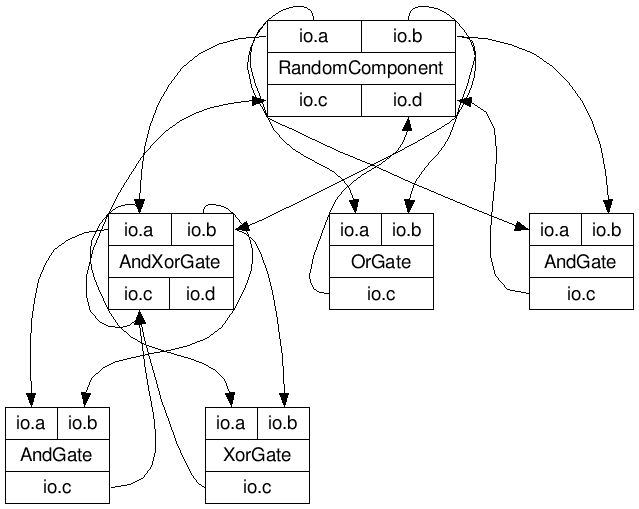
\includegraphics[width=0.7\textwidth]{img/HierarchicalLayoutSimple}
  }
  \caption[Simple hierarchical layout for diagram visualization]{The simplest
    hierarchical visualization, where parents are just represented using various
    heights}
  \label{fig:hierarchical-layout-simple}
\end{figure}

The problem by using such a representation is clearly visible, sometimes the
ports of a component is an output type port as well as an input type port.
This can be seen at the port "io.c" from the \texttt{AndXorGate} component. In
listing \ref{lst:andxorgate-problem}, we can see that the value \verb|io.c| is
written as an output of the component. In the figure
\ref{fig:hierarchical-layout-simple}, the same port is the source and the target
of some connections. This can cause some misunderstanding.

\begin{listing}[H]
  \centering
\begin{scalacode}
class AndXorGate extends Component {

  val xorGate = new XorGate
  val andGate = new AndGate

  val io = new Bundle {
    val a: Bool = in Bool
    val b: Bool = in Bool
    val c: Bool = out Bool
    val d: Bool = out Bool
  }

  xorGate.io.a := io.a
  xorGate.io.b := io.b
  andGate.io.a := io.a
  andGate.io.b := io.b

  io.c := xorGate.io.c
  io.d := andGate.io.c
}
\end{scalacode}
  \caption[The AndXorGate component written with SpinalHDL]{The AndXorGate
component writtent with SpinalHDL. We can see that the ``c'' port is an output
of the components and in figure \ref{fig:hierarchical-layout-simple} the port is
shown as an input port and as an output port.}
  \label{lst:andxorgate-problem}
\end{listing}

\subsection{Tree view}

The idea of the tree view is to represent the hierarchical relation like in file
explorer. The figure \ref{fig:tree-view} depicts the idea for a SpinalHDL
component.

\begin{figure}[H]
  \centering
  \fbox{
    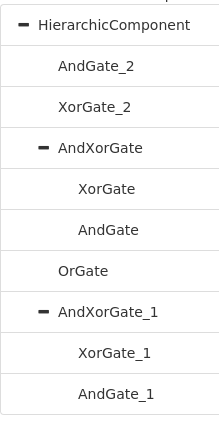
\includegraphics[width=0.2\textwidth]{img/tree-view}
  }
  \caption[SpinalHDL's Component visualization with tree view]{A tree view
    visualization of a SpinalHDL component, each child is under his parent and
    eventually possesses itself some sub-components.}
  \label{fig:tree-view}
\end{figure}

The tree view visualization is very useful to directly detect the relation
between some components. The big problem is that we can't see the connection
relationships.

\subsection{Multiple diagrams}

As seen with the hierarchical layout figure
\ref{fig:hierarchical-layout-simple}, the problem is that sometimes a port is an
output for some components and, in the other way, an input for some other
ones. If we look closely to the problem we could notice that a port receive
connections from her brothers and send connections to her childrens.

\begin{figure}[H]
  \centering
  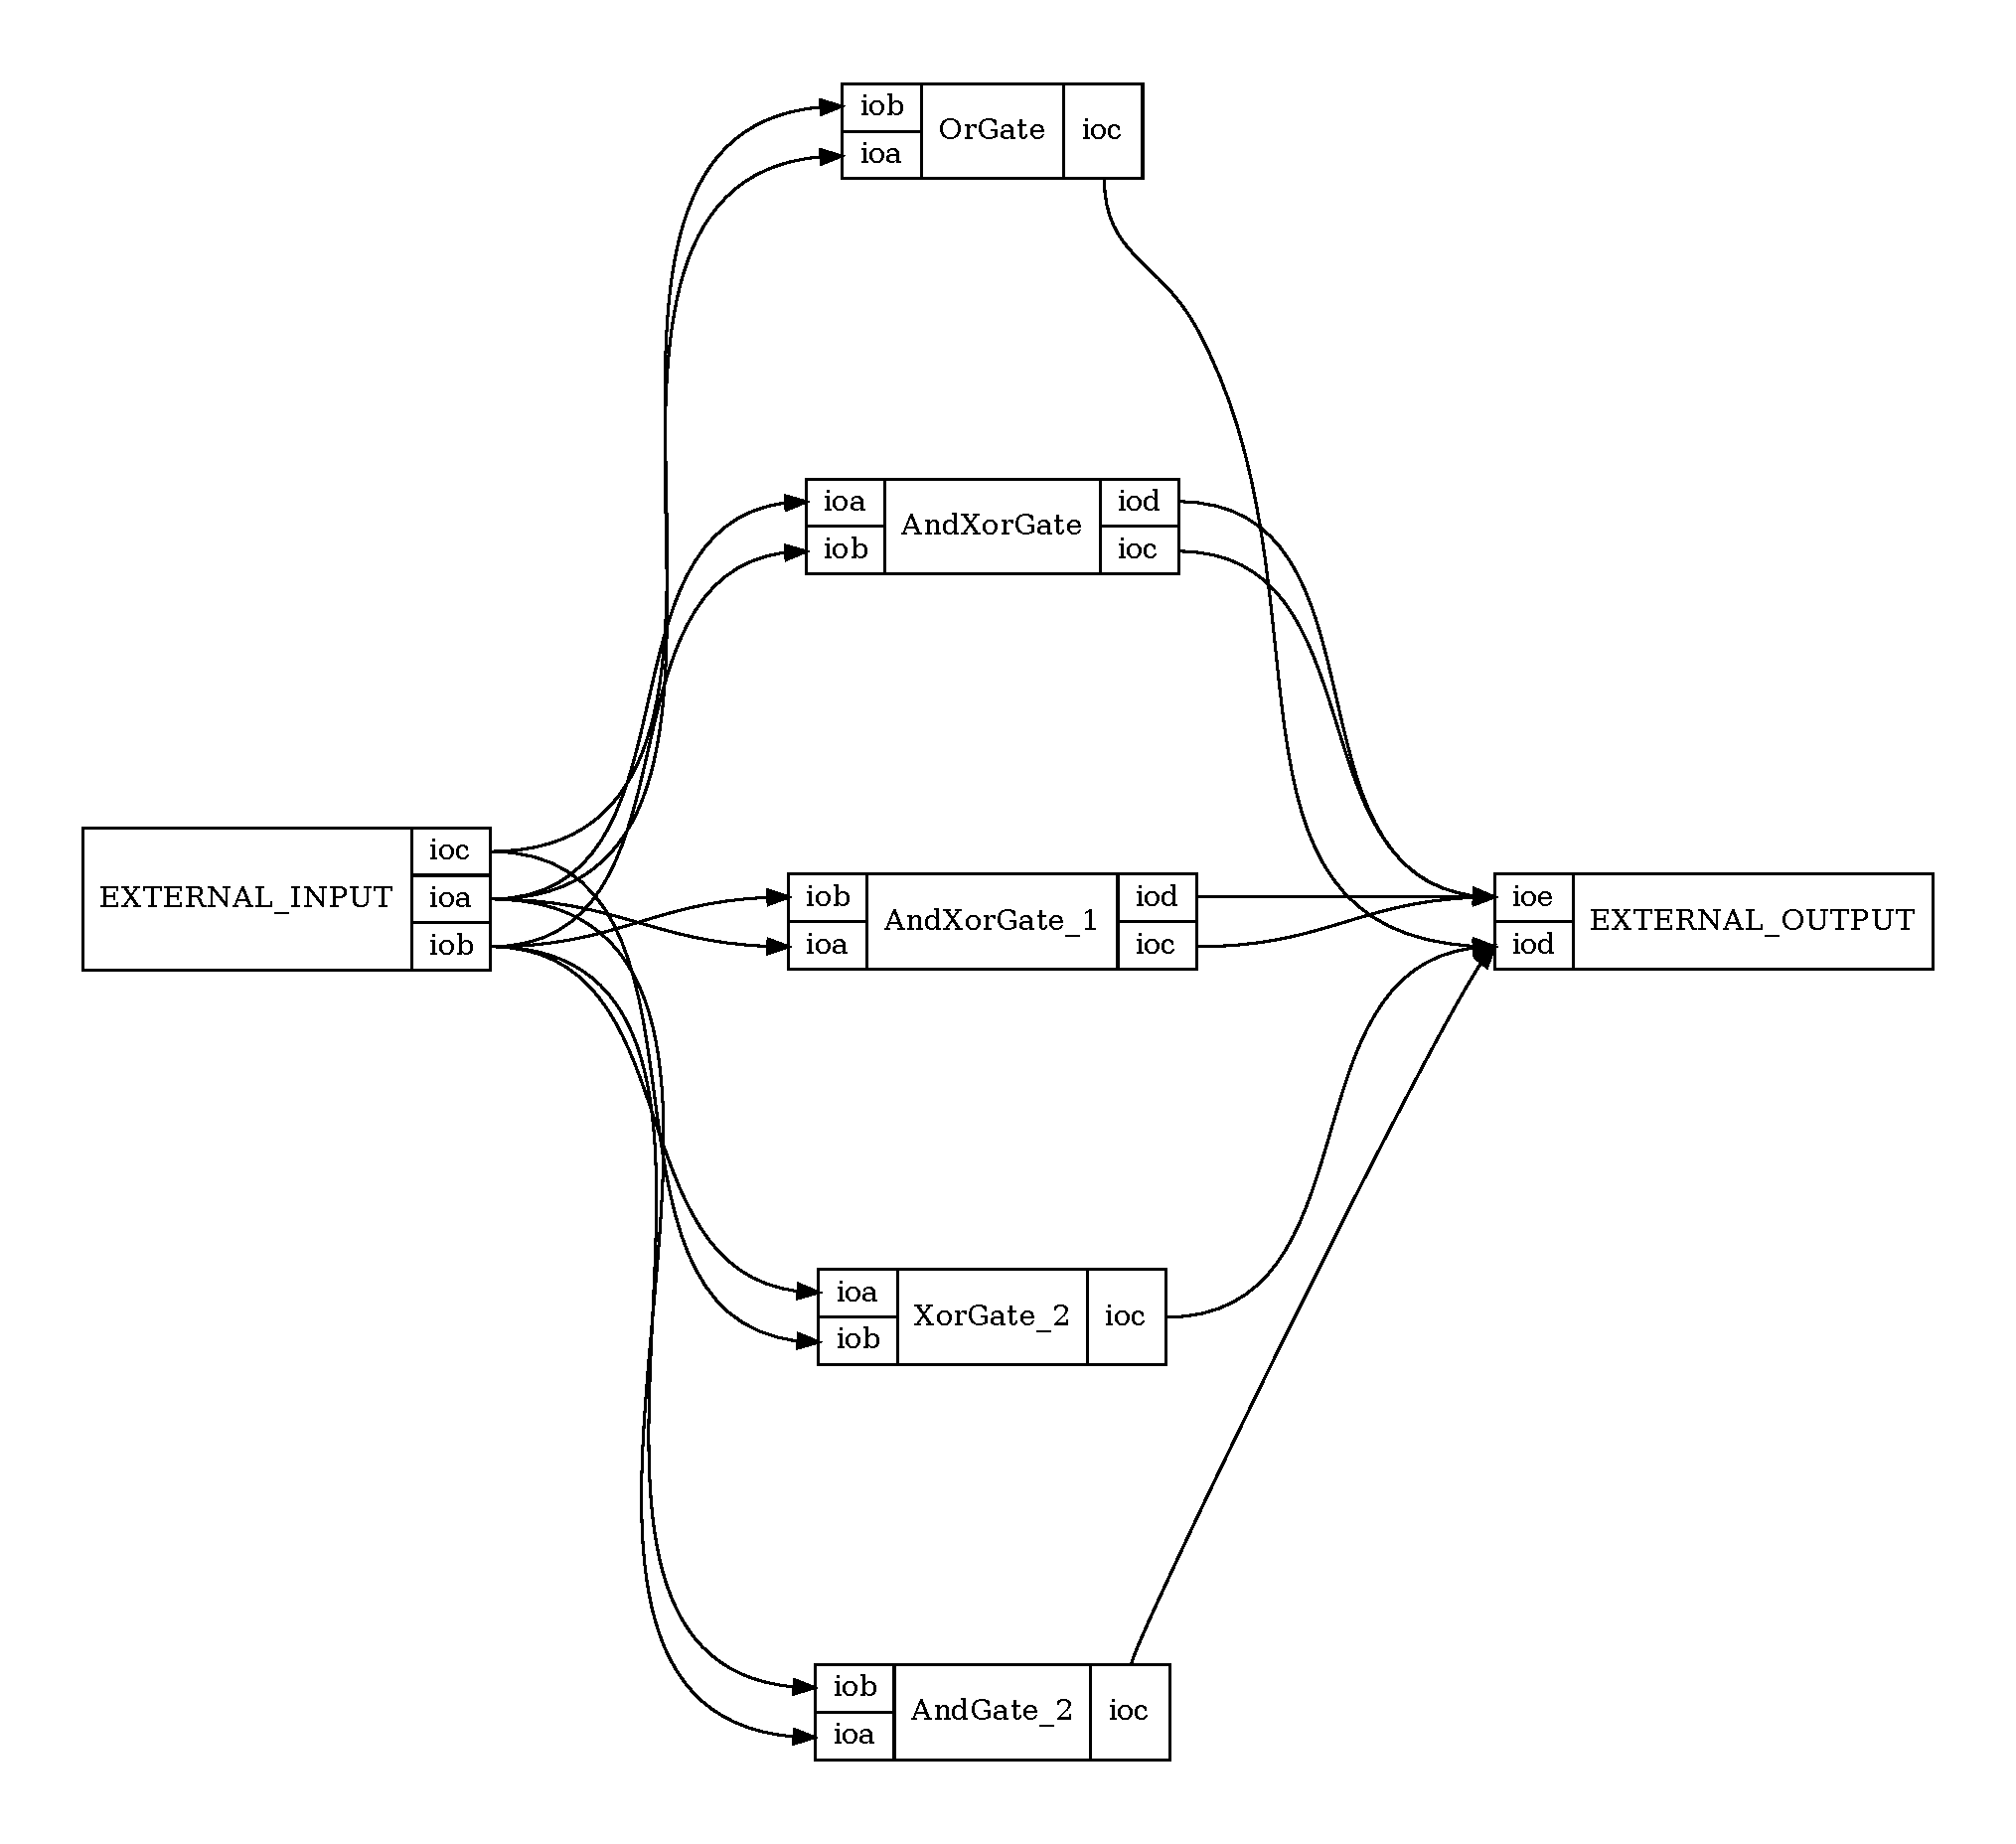
\includegraphics[width=0.6\textwidth]{img/HierarchicComponent.pdf}
  \caption[SpinalHDL Component inside]{Inside of a SpinalHDL component, the
    component possesses inputs and outputs as his own interface and communicates
  with her children}
  \label{fig:hierarchic-component}
\end{figure}

\begin{figure}[H]
  \centering
  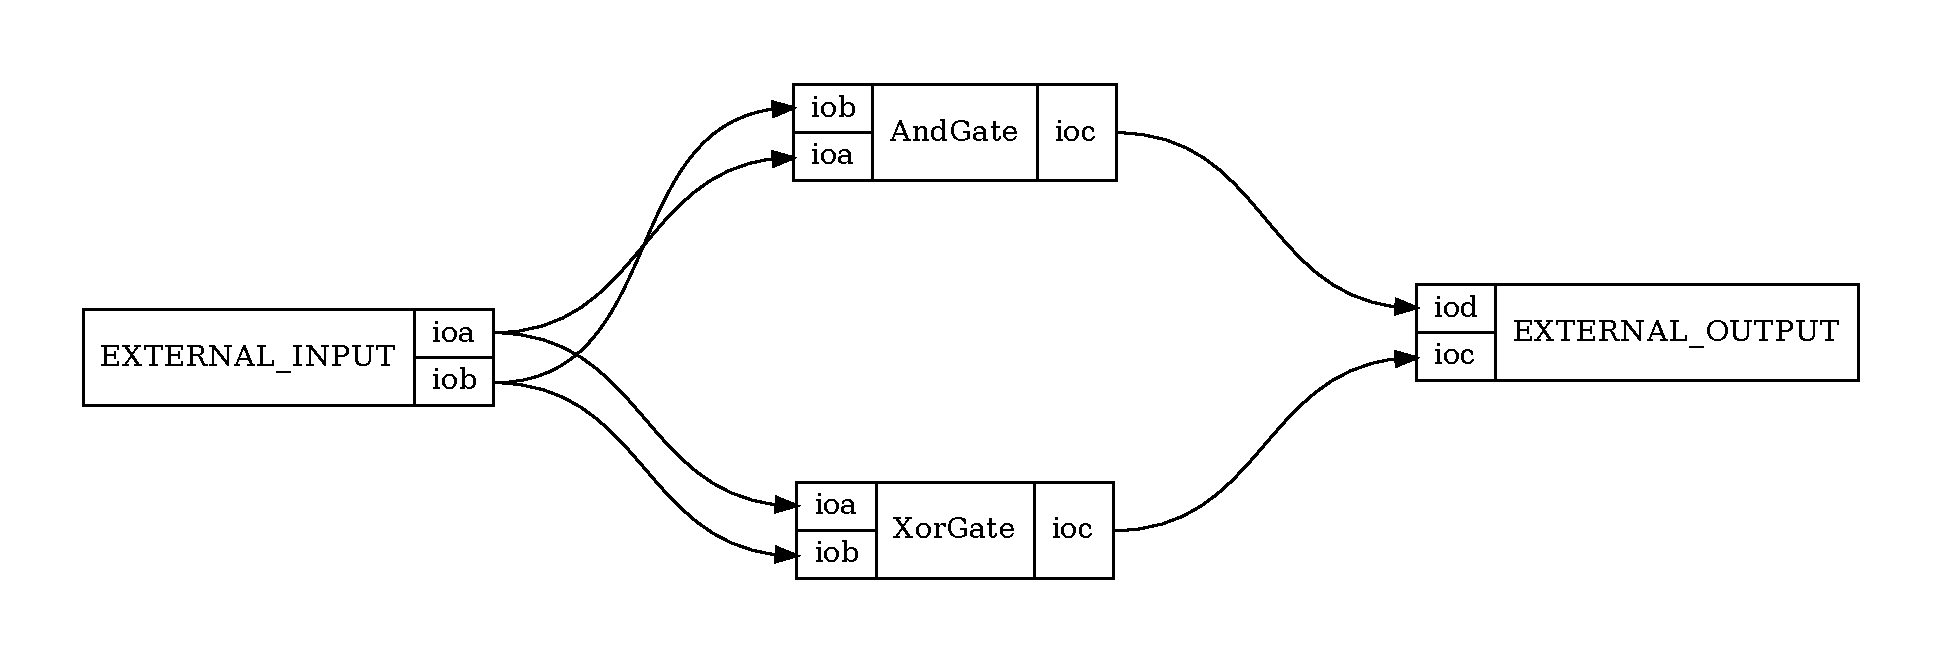
\includegraphics[width=0.6\textwidth]{img/AndXorGate.pdf}
  \caption[SpinalHDL Component inside an another]{Component which is the
    sub-component of the component from figure \ref{fig:hierarchic-component},
    the external inputs and outputs corresponding to the ones in the parent component}
  \label{fig:and-xor-gate}
\end{figure}

Using such a representation solve the problem discuss in
\ref{sec:hierarchical-layout} : if we represent all the components just using
one diagram, sometimes the ports are inputs and sometimes they are outputs. With
multiple diagram this problem no longuer occurs.

The major disadvantage is that we need an interactive diagram for exploring
the children of a component or multiple static ones which is not practical.

\section{A visual example}

The diagram we want to produce, as explained in chapter \ref{sec:graph-layout}, owns the following properties :
\begin{itemize}
  \item Oriented
  \item Cyclic
  \item Connection between ports on nodes and not between nodes
\end{itemize}

\section{Model representation}
\label{sec:model-representation} 

The model representation is builded using the oriented-object paradigm. The
figure \ref{fig:model-class-diagram} shows the class diagram of the models.

\begin{figure}[H]
  \centering
  \fbox{
  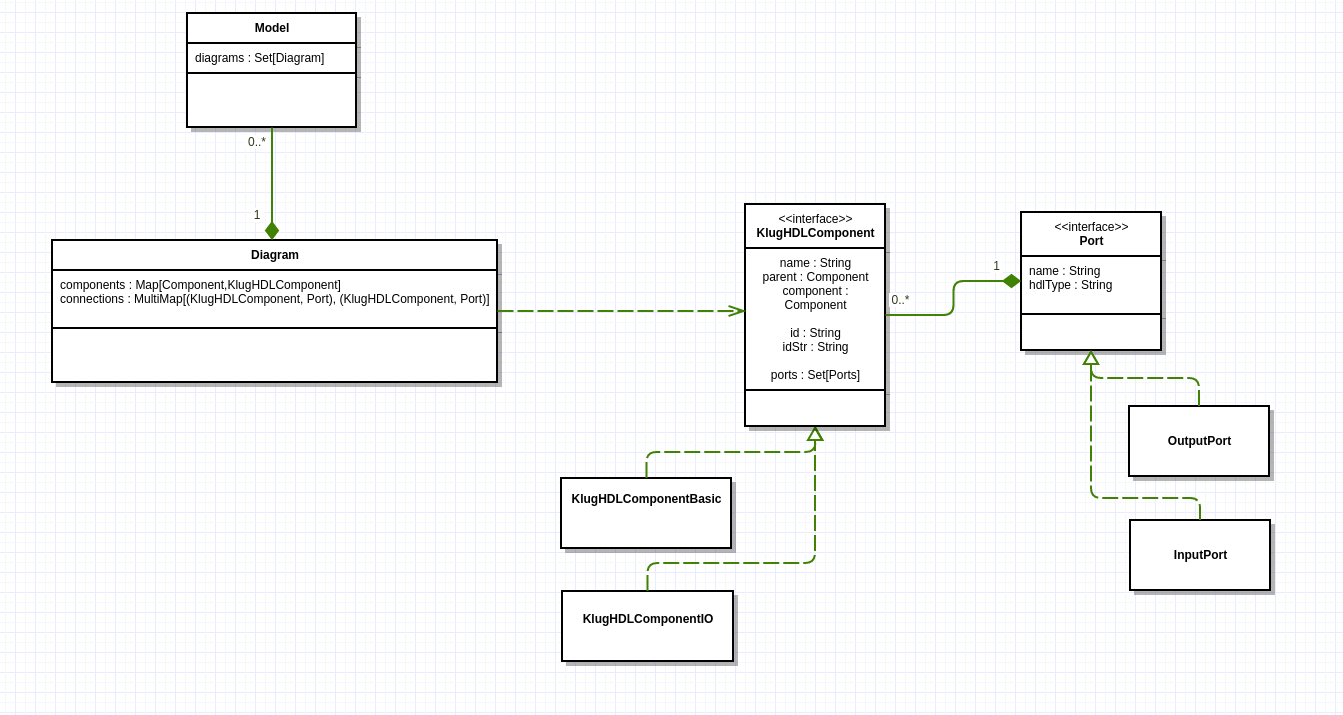
\includegraphics[width=0.99\textwidth]{img/class-diagram-intermeditate-model}
  }
  \caption[Class diagram of the intermediate model]{The complete class diagram of the intermediate model representation}
  \label{fig:model-class-diagram}
\end{figure}

\section{Conclusion}

The major advantage of such an intermediate representation is the capability to
evolve the program in order to produce additional outputs. For now there is just
a \textbf{DOT} and \textbf{JSON} backend. It also provides a way to check the
correctness of the diagram after the parsing on the AST : connections with
non-existing port for example.

%%% Local Variables:
%%% mode: latex
%%% TeX-master: "../report"
%%% End:

\chapter{Viewing library}
\label{cha:Viewing library}

This chapter will present some visualization library which could be used to
generate and interact with the component diagram. The comparison between those
library is based on the features we want to offer to the KlugHDL user (see
chapter \ref{sec:Goal}). In order to compare those viewing libraries, we end by
discuting the point of the evaluation and the evaluation of all the library
mentionned.

For the presentation of each of those libraries for graph visualization, we would
use the same graph showed in figure \ref{fig:graph-base-model}.

\begin{figure}[H]
  \centering
  \fbox{
    \digraph[scale=0.5]{GraphBaseModel}{
      node [shape=record];
      graph [rankdir=LR,
      ranksep="1",
      nodesep="1"];
      AndGate [label="{{<a>io.a : Bool|<b>io.b : Bool}|AndGate|{<c>io.c : Bool}}"];
      OrGate [label="{{<a>io.a : Bool|<b>io.b : Bool}|OrGate|{<c>io.c : Bool}}"];
      Input [label="{Input|{<a>io.a : Bool|<b>io.b : Bool}}"];
      Output [label="{{<c>io.c : Bool}|Output}"];
      Input:a -> AndGate:a;
      Input:b -> AndGate:b;
      Input:a -> OrGate:a;
      Input:b -> OrGate:b;
      OrGate:c -> Output:c;
      AndGate:c -> Output:c;
    }
  }
  \caption[Graph model for the viewing library comparison]{The graph we will use
    in order to compare several viewing library. This model includes two
    logical components : a AND and a OR gate and two nodes which are
    representing the input and output of the parent component.}
  \label{fig:graph-base-model}
\end{figure}

\section{GraphStream}
\label{sec:GraphStream}

GraphStream is a Java library used for the modelisation and analysis of dynamic
graphs\cite{graphstream}. The goal of the library is to provide a way to
represents graphs and work on it\cite{graphstream}. GraphStream is an active
project hosted by the University of Le Havre in France.

\subsection{Implementation of the base graph model}
\label{sub:Implementation}

The figure \ref{fig:base-graph-model-graphstream} show the base graph model
realized with the GraphStream library.

\begin{figure}[H]
  \centering
  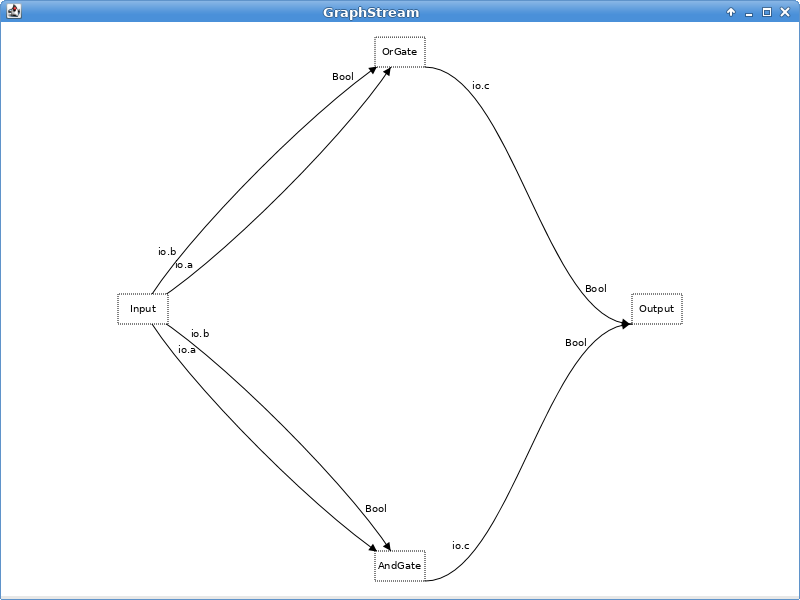
\includegraphics[width=0.8\textwidth]{img/graphstream-base-model-example}
  \caption{The base graph model rendering using Graphstream}
  \label{fig:base-graph-model-graphstream}
\end{figure}

GraphStream allow us to simply create a graph (or a multigraph) in Java like in
listing \ref{lst:graphstream-example}.

\begin{listing}[H]
  \centering
  \begin{javacode}
  Graph graph = new SingleGraph("Example");
  graph.addNode("A" );
  graph.addNode("B" );
  graph.addNode("C" );
  graph.addEdge("AB", "A", "B");
  graph.addEdge("BC", "B", "C");
  graph.addEdge("CA", "C", "A");
  \end{javacode}
  \caption[A simple graph modelisation using GraphStream]{Modelisation of a
    simple graph using the GraphStream library}
  \label{lst:graphstream-example}
\end{listing}

\subsection{Remarks}
\label{sub:Remarks}

With GraphStream, there is no way to control some visual features which are very
interesting for hardware component visualization : the splines of the edges and
the anchor position on the node. There is no way to have a node with sub-node
like in the base graph model in figure \ref{fig:graph-base-model}.

An additional special case is the label on the edges. With GraphStream, we could
add some labels on the edges like in listings \ref{lst:graphstream-edge-label},
but we can't add multiple ones. To add multiple labels we need to use sprite like
in listing \ref{lst:graphstream-edge-sprite}.

\begin{listing}[H]
  \centering
  \begin{javacode}
  Graph graph = new MultiGraph("Edges label example");
  graph.addAttribute("ui.quality");
  graph.addAttribute("ui.antialias");
  
  graph.addNode("A");
  graph.addNode("B");
  Edge edge = graph.addEdge("AB", "A", "B", true);
  edge.addAttribute("ui.label", "A --> B");
  graph.display(false);
  \end{javacode}
  \caption[Add a label on an edge with GraphStream]{A complete example on how to
add a label to an edge with the GraphStream library.}
  \label{lst:graphstream-edge-label}
\end{listing}

\begin{listing}[H]
  \centering
  \begin{javacode}
    SpriteManager sman = new SpriteManager(graph);

    // add label 1
    Sprite label1 = sman.addSprite("label1");
    label1.attachToEdge("AB");
    label1.setPosition(0.2, 0, 0);
    label1.addAttribute("ui.label", "Label 1");
    label1.addAttribute("ui.style", "fill-mode:none;");

    // add label 2
    Sprite label2 = sman.addSprite("label2");
    label2.attachToEdge("AB");
    label2.setPosition(0.8, 0, 0);
    label2.addAttribute("ui.label", "Label 2");
    label2.addAttribute("ui.style", "fill-mode:none;");
  \end{javacode}
  \caption[Add two label on an edge with GraphStream]{A complete example on how
to add multiples labels to an edge with the GraphStream library. This time, we
need to use sprites.}
  \label{lst:graphstream-edge-sprite}
\end{listing}

\subsection{Conclusion}
\label{sub:Conclusion-gs}

GraphStream owns other features which could be useful to design an application :
\begin{itemize}
\item View integration using Swing
\item Human-Computer interaction with the view
\item A complete CSS interpretation to personalize the nodes and the edges
\end{itemize}

The main problem using GraphStream is that we need to indicate the component
information using label on the edges. The figure
\ref{fig:base-graph-model-graphstream} show four nodes and six connections, but
if we have a lot more edges between nodes, it would be difficult to see the
type of the inputs and outputs, shown in figure
\ref{fig:graphstream-lot-of-edges}.

\begin{figure}[H]
  \centering
  \fbox{
    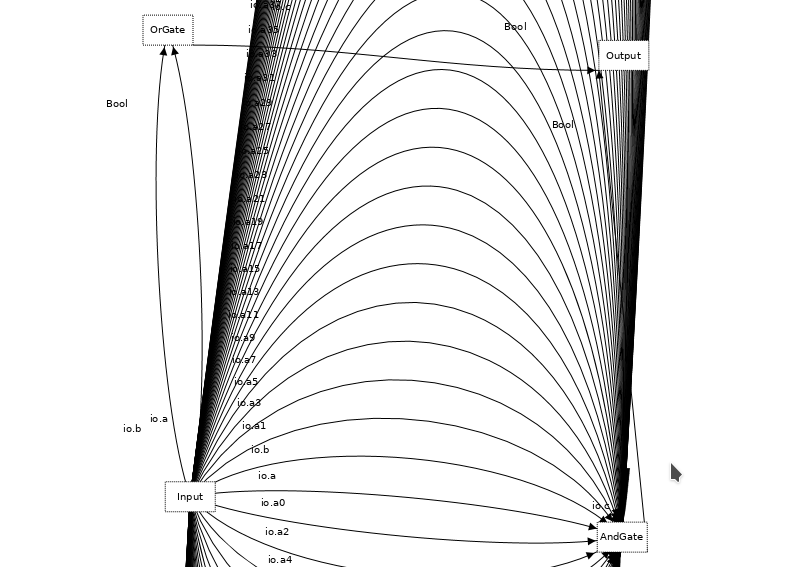
\includegraphics[width=0.8\textwidth]{img/graphstream_lot_of_edges}
  }
  \caption[Label on multiple edges using GraphStream]{}
  \label{fig:graphstream-lot-of-edges}
\end{figure}

In order to overpass those problem, we need to visualize the type in an another
form : in the graph \ref{fig:graph-base-model} we have the idea to show the
inputs and outputs as a port of the component. With GraphStream we can't do
it, so we need an another library which have this idea of port.

\section{Draw2D}
\label{sec:Draw2D}

Draw2D is a HTML5 and Javascript library for visualization and interaction with
diagrams and graphs\cite{draw2d}. The goal of the library is to provide a way to
represent diagrams and graphs and manipulate those using the mouse or Javascript
code. Some existing product already use Draw2d for diagrams manipulation :

\begin{itemize}
\item Shape Designer\cite{draw2d}
\item BrainBox\cite{draw2d}
\item Sankey State\cite{draw2d}
\end{itemize}

\subsection{Implementation of the base graph model}
\label{sub:Implementation of the base graph model}

Before implementing directly the basic example of the graph \ref{fig:graph-base-model},
we need to extend the library with a new component for our usage.
In the chapter \ref{sub:Conclusion-gs} we indicate that the GraphStream library is lacking the idea of port, but Draw2d already have them.

The listing \ref{lst:draw2d-base-graph-model} shows the realisation of the base
graph model example. Note that the object \textbf{ComponentShape} and the
functions \textbf{ComponentShape.addPort()},\textbf{newConnection()} and
\textbf{createConnection()} are not part of the Draw2d library, it's an
extension added for this project.

The code \ref{lst:draw2d-base-graph-model} is producing the HTML page see in
figure \ref{fig:base-graph-model-html-draw2d}.

\begin{listing}[H]
  \centering
  \begin{jscode}
    var canvas = new draw2d.Canvas("gfx_holder1");

    var andGate = new ComponentShape();
    var orGate = new ComponentShape();
    var input = new ComponentShape();
    var output = new ComponentShape();

    canvas.installEditPolicy(new draw2d.policy.connection.DragConnectionCreatePolicy({
      createConnection: createConnection
    }));

    andGate.setName("AndGate");
    orGate.setName("OrGate");
    input.setName("Input");
    output.setName("Output");

    andGate.addPort("io.a", "input");
    andGate.addPort("io.b", "input");
    andGate.addPort("io.c", "output");

    orGate.addPort("io.a", "input");
    orGate.addPort("io.b", "input");
    orGate.addPort("io.c", "output");

    input.addPort("io.a", "output");
    input.addPort("io.b", "output");

    output.addPort("io.c", "input");

    canvas.add(input);
    canvas.add(output);
    canvas.add(andGate);
    canvas.add(orGate);

    canvas.add(newConnection(input.getPort("io.a"), andGate.getPort("io.a")));
    canvas.add(newConnection(input.getPort("io.b"), andGate.getPort("io.b")));
    canvas.add(newConnection(input.getPort("io.a"), orGate.getPort("io.a")));
    canvas.add(newConnection(input.getPort("io.b"), orGate.getPort("io.b")));
    canvas.add(newConnection(andGate.getPort("io.c"), output.getPort("io.c")));
    canvas.add(newConnection(orGate.getPort("io.c"), output.getPort("io.c")));
  \end{jscode}

  \caption[Base graph model implementation using the Draw2D library]{The necessary code to produce the base graph model with the Draw2d library.
    The object \textbf{ComponentShape} and the functions \textbf{addPort()},
    \textbf{newConnection()} and \textbf{createConnection()} are not part of the
    Draw2d library, it's an extension added for this project.}
  \label{lst:draw2d-base-graph-model}
\end{listing}


\begin{figure}[H]
  \centering
  \fbox{
    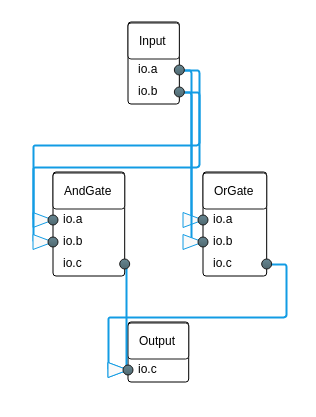
\includegraphics[width=0.3\textwidth]{img/draw2d-base-model-example}
  }
  \caption[Render of the base graph model using the Draw2D library]{Rendering of
    the base graph model diagram from figure \ref{fig:graph-base-model} using
    the Draw2D library}
  \label{fig:base-graph-model-html-draw2d}
\end{figure}

\section{Graph layout}
\label{sec:graph-layout}

A feature that Draw2D doens't owns is the layout of the diagram. If we did not
say anything about the position of the node, Draw2D simply overlaps all the nodes
and manages nothing for the visualization as illustrate in figure
\ref{fig:draw2d_overlapping}.

\begin{figure}[H]
  \centering
  \fbox{
    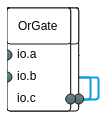
\includegraphics{img/overlap_draw2d}
  }
  \caption[Overlapping of nodes by Draw2D]{When we specify nothing about the
    node position with Draw2D, the engine just overlaps all the nodes.}
  \label{fig:draw2d_overlapping}
\end{figure}

In order to produce a visualisable diagram, we need to layout ourself the
diagram. We need to mention that's the layout algorithm is a NP-Hard problem in
computing theory\cite{Tamassia:2007:HGD:1202383} and for our graph, we have some
specialties :

\begin{itemize}
\item The graph could be cyclic
\item The graph is oriented
\item Nodes owns port, so we need to layout the edges on specific part of the graph
\end{itemize}

The first two specialties aren't a big deal, but the last one is quite
problematic, it involved a special layout algorithm which take care of the ports
position on the nodes. Otherwise the visual result could be chaotic like in
figure \ref{fig:multigraph-no-port}, in which we can't see the connections
between some specific ports.

\begin{figure}[H]
  \centering
  \fbox{
    \digraph[scale=0.5]{MultiGraphNoPort}{
      A -> B -> C -> D;
      A -> B -> C;
      A -> B;
      D -> A;
      D -> B;
    }
  }
  \caption[Visualization of a multi-graph without port]{Visualization of a
    multi-graph without port, we could not determine the connection which is
    representing a certain connection between two components.}
  \label{fig:multigraph-no-port}
\end{figure}

In order to solve this drawback, we need to layout the graph ourself by using a
library. We could also do it ourselves by implementing the algorithm for the kind
of graph we have, but it's too time-consuming for a project like this.

\section{Conclusion}
\label{sec:viewing-library-conclusion}

GraphStream looks like a really good library for manipulating graphs and visualize
them. The problem is that there is no good way to visualize the ports of the
components so we have to labelize the connections and it looks ugly (figure
\ref{fig:graphstream-lot-of-edges}). Then we have to find a library which allows
this idea of ports. We find them with Draw2D and choose it for the project. The
disadvantage of using this library is that we can't layout easily the graph by
ourselves.

%%% Local Variables:
%%% mode: latex
%%% TeX-master: "../report"
%%% End:
\chapter{Parsing the AST}
\label{chap:parsing-ast}

The abstract syntax tree of SpinalHDL is the core components of all the KlugHDL
product. He is used to produce the intermediate representation in the generation
pipeline (figure \ref{fig:generation-pipeline}) and once the intermediate
representation is built, the rest is easely makable.

The concept of AST as already been explain in chapter \ref{sub:Abstract Syntax
  Tree}. Using this, we are going to see the parsing of the SpinalHDL AST in
order to generate an intermediate model. The parsing and the following
generation into the intermediate model is separate in multiple
phases :

\begin{itemize}
\item Diagram parsing
\item Components parsing
\item Ports parsing
\item Connections parsing
\end{itemize}

As illustrate in the intermediate model class diagram
\ref{fig:model-class-diagram}, the intermediate representation is composed like
the following :
\begin{itemize}
\item A model possesses multiple diagrams (at least two : the toplevel and the
  root component)
\item A diagrams possesses at least one component with zero or more ports
\item A diagrams possesses zero or more connections which are 
\end{itemize}

A model could be represented, using scala, with the class declaration in listing
\ref{lst:model-scala}. A model is a set of diagrams which are related to a
toplevel component.

\begin{listing}[H]
  \centering
  \begin{scalacode}
    case class Model(topLevel : Component) {

      var diagrams : Set[Diagram] = Set()
  }
\end{scalacode}
\caption[Model class declaration]{Declaration of the model with scala, a model
  is basically a set of diagrams and is attached to a topLevel component, which
  is the only component of the AST which as no parent}
\label{lst:model-scala}
\end{listing}

\section{Diagram parsing}
\label{sec:diagrams-parsing}

Generating a diagram (see listing \ref{lst:diagram-scala}) is trivial because we
just have to retrieve all the components which are parents, the algorithm is
implemented in listing \ref{lst:generate-diagram}. 
\begin{listing}[H]
  \centering
  \begin{scalacode}
    class Diagram(val parent : Component) {

      var components : Map[Component, KlugHDLComponent] = Map()
      var connections : mutable.MultiMap[
          (KlugHDLComponent,Port),
          (KlugHDLComponent, Port)
        ]
      }
  \end{scalacode}
  \caption[Diagram class declaration]{Declaration of a the diagram class with
    scala, a diagram is a set of components (here as a Map) and a set of
    connections (here as a multimap for the orientation)}
  \label{lst:diagram-scala}
\end{listing}

\begin{listing}[H]
  \centering
  \begin{scalacode}
  def generateDiagrams(component : Component) : Unit = {
    diagrams += new Diagram(component.parent)
    component.children.foreach(generateDiagrams)
  }
  \end{scalacode}
  \caption[Parsing the diagrams form the AST]{This function parse the AST and
    generate all the corresponding diagrams object for a specific component}
  \label{lst:generate-diagram}
\end{listing}

Because we are using a set,
we don't have to check if the digrams already exist. To make this possible we
have to redifine the \verb|equals| function like in listing \ref{lst:diagram-equals-scala}.

\begin{listing}[H]
  \centering
  \begin{scalacode}
  override def equals(o : scala.Any) : Boolean = o match {
    case d : Diagram => this.parent == d.parent
    case _ => super.equals(o)
  }
  \end{scalacode}
  \caption[Equals function implementation for the Diagram Class]{We have to
    override the equals function in order to use the diagrams in a set as expected}
  \label{lst:diagram-equals-scala}
\end{listing}

\section{Components parsing}
\label{sec:components-parsing}

The parsing and generation of the components is made for each diagrams one by
one. Here, the algorithm is quite simple too. The algorithm is implemented in
the listing \ref{lst:component-parse-scala} and the KlugHDLComponent is declared
in listing \ref{lst:component-scala}.

\begin{listing}[H]
  \centering
  \begin{scalacode}
  sealed trait KlugHDLComponent {

    val name : String
    val parent : Component
    val component : Component = this match {
      case KlugHDLComponentBasic(_, c, _) => c
      case KlugHDLComponentIO(_, _) => null
    }
  }

  final case class KlugHDLComponentBasic(name : String, override val component : Component, parent : Component) extends KlugHDLComponent

  final case class KlugHDLComponentIO(name : String, parent : Component) extends KlugHDLComponent
  \end{scalacode}
  \caption[Diagram class declaration]{Declaration of the Components class (here
    names KlugHDLComponents). There is two type of components : the basic ones
    and the ones who represent the external world input and output like in
    figure \ref{fig:and-xor-gate}}
  \label{lst:component-scala}
\end{listing}

\begin{listing}[H]
  \centering
  \begin{scalacode}
  private def generateComponent(diagram : Diagram) : Model = {
    diagram.foreachChildren(diagram.addComponents, topLevel)
    if (diagram.parent != null)
      diagram.addIoComponents(diagram.parent)
    this
  }

  def addComponents(component : Component) : Unit = {
    components += (component -> KlugHDLComponentBasic(component.definitionName, component, component.parent))
  }
  
  def addIoComponents(component : Component) : Unit = {
    if (component == null)
      components += (component -> KlugHDLComponentIO("NULL", component))
    else
      components += (component -> KlugHDLComponentIO(component.definitionName, component))
  }
  \end{scalacode}
  \caption[Implementation of the components parsing]{Components parsing and
    generation in scala for one diagram}
  \label{lst:component-parse-scala}
\end{listing}

Note that we generate the interface for the external world connections in the
model. This two KlugHDLComponentIO aren't present in the SpinalHDL AST.

\section{Ports parsing}
\label{sec:ports-parsing}

The ports generation is, again, easy to make. In the SpinalHDL model, the
Components class already ownes a \verb|getAllIo| function which return all the
inputs and outputs node for a components. So we just need to create a ports
object (listing \ref{lst:port-scala}) from these and add it to the correct
KlugHDLComponents. The algorithm is implement in the listing
\ref{lst:port-parsing-scala}.

\begin{listing}[H]
  \centering
  \begin{scalacode}
  sealed trait Port {

    val name : String
    val hdlType : String
  }

  final case class InputPort(name : String, hdlType : String) extends Port

  final case class OutputPort(name : String, hdlType : String) extends Port
  \end{scalacode}
  \caption[Diagram class declaration]{Declaration if the Port class with scala,
    there is two types of ports : input and output}
  \label{lst:port-scala}
\end{listing}

\begin{listing}[H]
  \centering
  \begin{scalacode}
  def generatePort(diagram: Diagram): Unit = {
    def generatePort(entry: (Component, KlugHDLComponent)): Unit = {
      if (entry._1 != null) {
        entry._1.getAllIo.foreach { bt =>
          entry._2.addPort(Port(bt))
        }
      }
    }

    diagram.components.foreach(generatePort)
  }
  \end{scalacode}
  \caption[Implementation of the ports parsing]{Ports parsing and generation in
    scala for one diagrams, the ports are generating component by component}
  \label{lst:port-parsing-scala}
\end{listing}

\section{Connections parsing}
\label{sec:connections-parsing}

The connections parsing is the hardest implementation to do. The reason is we
have multiple type of connections :
\begin{itemize}
\item input connections
\item output connections
\item input connections from parent
\item output connections from parent
\end{itemize}

In addition, to find the staring point of a connection, we have to parse
recursively all the nodes of the AST until we found a \verb|Basetype| object
which is the type for the inputs and outputs nodes of a SpinalHDL component.

\subsection{Input connections}
\label{sec:input-connections}

The input connections represent all the connections generated romom the inputs of a
nodes. Firstable, we have to retrieve all the inputs for a specific AST nodes
then we need to generate a connections between two ports on two nodes. The
implementation could be seen in listing \ref{lst:parse-input-connection-scala}.

\begin{listing}[H]
  \centering
  \begin{scalacode}
  def parseInputConnection(component: Component): Unit = {
      
    def parseInputs(node: Node): List[BaseType] = {
      
      // iterate over all the inputs on each nodes of the AST until founding an
      // output basetype
      def inner(node: Node): List[BaseType] = node match {
        case bt: BaseType =>
          if (bt.isOutput) List(bt)
          else List(bt) ::: node.getInputs.map(inner).foldLeft(List(): List[BaseType])(_ ::: _)
        case null => List()
        case _ => node.getInputs.map(inner).foldLeft(List(): List[BaseType])(_ ::: _)
      }

      inner(node).filter {
        _ match {
          case bt: BaseType => bt.isOutput
          case _ => false
        }
      }
    }

    for {
      io <- component.getAllIo
      if io.isInput
      input <- parseInputs(io)
    } {
      diagram.addConnection(input.component, Port(input), io.component, Port(io))
    }
  }
  \end{scalacode}
  \caption[Parsing and generation of the inputs connections]{Implementation in
    scala of the parsing and generation for all the inputs connections for a
    specific component}
  \label{lst:parse-input-connection-scala}
\end{listing}

\subsection{Output connections}
\label{sec:output-connections}

The output connections represent all the connections generated from the outputs
of a node. The problem is the same as for the input connections but in the other
way : we need to parse the consumer for a specific node like in listing.

\begin{listing}[H]
  \centering
  \begin{scalacode}
  def parseOutputConnection(component: Component): Unit = {
      
    def parseConsumers(node: Node): List[BaseType] = {
      
      // iterate over all the inputs on each nodes of the AST until founding an
      // input basetype
      def inner(node: Node): List[BaseType] = node match {
        case bt: BaseType =>
          if (bt.isInput) List(bt)
          else List(bt) ::: node.consumers.map(inner).foldLeft(List(): List[BaseType])(_ ::: _)
        case null => List()
        case _ => node.consumers.map(inner).foldLeft(List(): List[BaseType])(_ ::: _)
      }

      inner(node).filter {
        _ match {
          case bt: BaseType => bt.isInput
          case _ => false
        }
      }
    }

    for {
      io <- component.getAllIo
      if io.isInput
      consumer <- parseConsumers(io)
    } {
      diagram.addConnection(io.component, Port(io), consumer.component, Port(consumer))
    }
  }
  \end{scalacode}
  \caption[Parsing and generation of the outputs connections]{Implementation in
    scalaof the parsing and generation for all the inputs connections for a
    specific component}
  \label{lst:parse-output-connection-scala}
\end{listing}

\subsection{Parent connections}
\label{sec:parent-connections}

Finally we could parse and generate the connections with the parent. This part
is slightly easier than the two previous one. Because we just have to generate
the inputs and consumers and subtract them like in a set. The algorithm is
describe in listing \ref{lst:parse-parent-connection}.

\begin{listing}[H]
  \centering
  \begin{scalacode}
  def parseParentConnection(component: Component): Unit = {

    def parseInputParentConnection(component: Component): Unit = {
      if (component.parent != null) {
        val con = for {
          io_p <- component.parent.getAllIo
          io <- component.getAllIo
          if io.getInputs.contains(io_p)
        } yield (io_p.component, Port(io_p), io.component, Port(io))
        con.foreach(diagram.addConnection)
      }
    }

    def parseOutputParentConnection(component: Component): Unit = {
      if (component.parent != null) {
        val con = for {
          io_p <- component.parent.getAllIo
          io <- getInputs(io_p)
          if io != null
        } yield (io.component, Port(io), io_p.component, Port(io_p))
        con.foreach(diagram.addConnection)
      }
    }

    def getInputs(bt: BaseType): List[BaseType] = {
      val comp = bt.component

      def inner(n: Node, acc: List[Node]): List[Node] = {
        if (n == null) acc
        else if (n.component != comp) {
          acc
        }
        else if (n.getInputsCount > 1) {
          n.getInputs.flatMap(n => inner(n, Nil)).toList
        }
        else {
          inner(n.getInputs.next(), n :: acc)
        }
      }

      inner(bt, Nil).map(_.getInputs.next().asInstanceOf[BaseType])
  }

    parseInputParentConnection(component)
    parseOutputParentConnection(component)
  }
\end{scalacode}
  \caption[Parsing and generation of the connections with the
  parent]{Implementation in scala of the parsing and generation of all the
    connections (inpus and outputs ones) with the parent}
  \label{lst:parse-parent-connection}
\end{listing}

\section{Conclusion}
\label{sec:ast-parsing-conclusion}

The parsing of the AST is the hardest part to understand, there is a lot to know
about SpinalHDL itself and a large amount of special case to understand. By the
way, it's the most important part too, with the generation of the
intermediate model we could do all the rest.
\chapter{Diagram visualization}
\label{chap:diagram-visualization}

This chapter will present the visualization of the diagram. First, we will
introduce the intermediate model backend used by KlugHDL in order to produce an
output for further use. Then we will see the static and dynamic visualizations
which are available with KlugHDL.

\section{Intermediate representation}
\label{sec:intermediate-representation}

The intermediate representation generate after the AST parsing is an
object-oriented representation created for KlugHDL. In order to use the
generated diagrams in other software we need to produce a standard output. In
KlugHDL those additional output are called ``backend''.

\subsection{The DOT backend}
\label{sec:dot-backend}

DOT and Graphviz are two software for diagram visualization. The diagram is
written using the DOT language and then compiled to various image formats
like png or pdf.

The advantage of using DOT is the simplicity. The figure \ref{fig:dot-example-2}
shows a Graphviz diagram generated by the DOT program. The corresponding code is
available in listing \ref{lst:dot-example-2}.

\begin{figure}[H]
  \centering
  \fbox{
    \digraph[scale=0.4]{DotExample2}{
      node [shape=record];
      graph [rankdir=LR,
      ranksep="1",
      nodesep="1"];
      AndGate [label="{{<a>io.a : Bool|<b>io.b : Bool}|AndGate|{<c>io.c : Bool}}"];
      OrGate [label="{{<a>io.a : Bool|<b>io.b : Bool}|OrGate|{<c>io.c : Bool}}"];
      Input [label="{Input|{<a>io.a : Bool|<b>io.b : Bool}}"];
      Output [label="{{<c>io.c : Bool}|Output}"];
      Input:a -> AndGate:a;
      Input:b -> AndGate:b;
      Input:a -> OrGate:a;
      Input:b -> OrGate:b;
      OrGate:c -> Output:c;
      AndGate:c -> Output:c;
    }
  }
  \caption[Example of a Graphviz diagram]{A complete Graphviz diagram generated
    by DOT, the code of this example is available in listing \ref{lst:dot-example-2}}
  \label{fig:dot-example-2}
\end{figure}

\begin{figure}[H]
  \centering
  \begin{textcode}
    digraph g {
      node [shape=record];
      graph [rankdir=LR,ranksep="1",nodesep="1"];
      AndGate [label="{{<a>io.a : Bool|<b>io.b : Bool}|AndGate|{<c>io.c : Bool}}"];
      OrGate [label="{{<a>io.a : Bool|<b>io.b : Bool}|OrGate|{<c>io.c : Bool}}"];
      Input [label="{Input|{<a>io.a : Bool|<b>io.b : Bool}}"];
      Output [label="{{<c>io.c : Bool}|Output}"];
      Input:a -> AndGate:a;      Input:b -> AndGate:b;
      Input:a -> OrGate:a;       Input:b -> OrGate:b;
      OrGate:c -> Output:c;      AndGate:c -> Output:c;
    }
  \end{textcode}
  \caption[Example of a Graphviz program]{A complete example of a DOT program,
    the corresponding diagram is available in figure \ref{fig:dot-example-2}}
  \label{lst:dot-example-2}
\end{figure}

We could just notice that we use the \verb|shape=record| option of DOT in order
to generate the ports on the nodes and link them with the connection.

\subsection{The JSON backend}
\label{sec:json-backend}

JSON (JavaScript Object Notation) is a format mostly used by Javascript for
object serialization. The format is completely included in the Javascript
language which is able to directly understand the object notation without any
additional code to write.

At the beginning of the project, we tried to produce the Javascript
output directly from the intermediate model. The problem occurs we change
the library we are using, we need to change the entire backend. The solution is
to produce a JSON output, whatever which library we are using, the model would
always be the same.

For this backend we used the lift json library \cite{liftweb}. This library is
very easy to use and offer a small DSL in order to write readable code. The
listing \ref{lst:lift-example} shows an example of the lift json library to create a
KlugHDL component in JSON.

\begin{listing}[H]
  \centering
  \begin{scalacode}
  def generateJson(klugHDLComponent: KlugHDLComponent): JValue = klugHDLComponent match {
    case KlugHDLComponentBasic(name, _, _) =>
      ("name" -> name) ~
      ("type" -> "default") ~
      ("ports" -> klugHDLComponent.ports.map(generateJson))
    case KlugHDLComponentIO(name, _) =>
      ("name" -> name) ~
      ("type" -> "io") ~
      ("ports" -> klugHDLComponent.ports.map(generateJson))
  }
  \end{scalacode}
  \caption[Lift library example : a json DSL]{The lift json library offers the
    opportunity to write readable and scalable code with her DSL}
  \label{lst:lift-example}
\end{listing}

\section{Static visualization}
\label{sec:static-visualization}

With KlugHDL it's very simple to generate a diagram in a pdf format. For example, this could be
useful for a report documentation. The listing \ref{lst:dot-example-klughdl}
shows how to do it with a complete example.

\begin{listing}[H]
  \centering
  \begin{scalacode}
  /**
   * Example for generating pdf diagam with dot
   * of a SpinalHDL component
  **/
   
   object DotExample extends App {

    // Create the vhdl rtl
    val report = SpinalConfig(targetDirectory = "vhdl").generateVhdl(new SmallComponent)

    // generate the diagram
    Dot(targetDirectory = "dot").generatePDFDiagram(Model(report.toplevel))
  }
  \end{scalacode}
  \caption[KlugHDL example on how to generate a pdf diagram]{A complete KlugHDL
    example on how to generate a pdf diagram using the DOT backend}
  \label{lst:dot-example-klughdl}
\end{listing}

\section{Dynamic visualization}
\label{sec:dynamic-visualization}

A dynamic diagram visualization is also provided with KlugHDL. The listing
\ref{lst:json-example-klughdl} illustrates how to generate the json model for a
SpinalHDL component.

\begin{listing}[H]
  \centering
  \begin{scalacode}
  /**
   * Example for generating the json model
   * of a SpinalHDL component
   **/

   object JsonExample extends App {
     
     // Create the vhdl rtl
    val report = SpinalConfig(targetDirectory = "vhdl").generateVhdl(new SmallComponent)

     // generate the model
     Json(targetDirectory = "json").generateJsonModel(Model(report.toplevel))
   }
  \end{scalacode}
  \caption[KlugHDL example on how to generate a json model]{A complete KlugHDL
    example on how to generate a json model}
  \label{lst:json-example-klughdl}
\end{listing}

\subsection{Extending the draw2d library}
\label{sec:draw2d-impl}

We have to extend the draw2d library in order to create the specific diagram we
want. The only addition to make is to create another node for draw2d. This is
done by extending the \verb|VerticalLayout| shape. The whole new shape is
created with the code in listing \ref{lst:component-shape}.

\begin{listing}[p]
  \centering
  \begin{jscode}
    ComponentShape = draw2d.shape.layout.VerticalLayout.extend({
      NAME: "ComponentShape",
      init: function (attr) {
          var _this = this;
          this._super($.extend({
              bgColor: "#ffffff",
              color: "#000000",
              stroke: 1,
              radius: 3
          }, attr));
          this.classLabel = new draw2d.shape.basic.Label({
              text: "ClassName",
              stroke: 1,
              fontColor: "#000000",
              bgColor: "#ffffff",
              radius: this.getRadius(),
              padding: 10,
              resizeable: true,
              editor: new draw2d.ui.LabelInplaceEditor(),
              onDoubleClick: function () {
                  _this.doubleClickCallBack()
              }
          });
          this.add(this.classLabel);
      },
      setName: function (name) {
          this.classLabel.setText(name);
      },
      getName: function () {
          return this.classLabel.text;
      },
      getPort: function (name) {
          return this.getPorts().find(function (entry) {
              return entry.name == name
          });
      },
      addPort: function (name, type) {
          var _this = this;
          var label = new draw2d.shape.basic.Label({
              text: name,
              stroke: 0,
              radius: 90,
              bgColor: null,
              padding: {left: 10, top: 3, right: 10, bottom: 5},
              fontColor: "#000000",
              resizeable: true,
              onDoubleClick: function () {
                  _this.doubleClickCallBack()
              },
              editor: new draw2d.ui.LabelEditor()
          });

          var port = label.createPort(type);
          port.setName(name);

          this.add(label);

          return label;
      },
      doubleClickCallBack: function () {
          console.log("double click callback")
      },
    });
  \end{jscode}
  \caption[Component shape prototype of KlugHDL]{A new prototype in draw2d is
    created by extending the VerticalLayout shape, then we have to provide a
    function for creating additional stack element in the shape}
  \label{lst:component-shape}
\end{listing}

The whole code for parsing the json model and display it into a web page is
available in the source code of the project.

\subsection{Problems}
\label{sec:problems}

Currently, there is a problem with the navigation through the diagrams. The
navigation from parent to brothers is fine but in the other direction, from the
children to the parent, some components are, sometimes, calling the callback
method on the double click input multiple times. This creates, first, a very long
callback and then corrupt the memory and raise exceptions.

%%% Local Variables:
%%% mode: latex
%%% TeX-master: "../report"
%%% End:

\chapter{Conclusion}
\label{cha:Conclusion}

This project tries to offer an additional tool for SpinalHDL in order to
increase his popularity. Domain specific languages are more and more used in
computer software nowadays and KlugHDL could be described as a tool for
development and documentation.

Writing VHDL code over and over again seems to be painful and SpinalHDL tries to
make the developer life easier, but VHDL owns a lot of tools to increase
productivity. KlugHDL is the first ``tool'' of the whole world of SpinalHDL and
launches a new era for SpinalHDL and its believers.

KlugHDL is able to parse and generate static diagrams with DOT and Graphviz for
any simple SpinalHDL component. Components with bus or complex basetype, like
$Uint(n bits)$ aren't supported for the moment. KlugHDL is also here to
demonstrate that it is possible to generate diagrams from the SpinalHDL AST.

We have seen that parsing the AST could be tricky and sometimes really strange.
We need additionnal SpinalHDL Components and much deeper understanding of the
SpinalHDL AST in order to parse and generate all the possible components which
could be written.

There is a lot of work to do on KlugHDL in order to have a complete tool for
diagrams generation. It is not only about the visualization but also about the
kind of SpinalHDL components to parse.

Some other features and work can be add to KlugHDL :
\begin{itemize}
\item Integrate the diagram visualization to an integrated software development
  like Eclipse or Intellij for a live preview of the current work.
\item Generate the diagram without generating the whole RTL for a component.
\end{itemize}

I would like to sincerely thanks the following people, whitout whom this project
would have been impossible to realize :

\begin{itemize}
\item Professor Dr. Mudry Pierre-André, for coordinating and supporting me
\item Charles Papon, author of SpinalHDL, for answered my questions about
  SpinalHDL and supporting me
\item Roland Julmy, my father, for having review this document and encouraging me.
\end{itemize}

Fribourg, the 17th January 2017

Sylvain Julmy

\chapter*{Sworn declaration}

`` I hereby solemnly declare that I have personally and independently prepared
this paper. All quotations in the text have been marked as such, and the paper
or considerable parts of it have not previously been subject to any examination
or assessment.''

\listoffigures
\listoflistings

%%% Local Variables:
%%% mode: latex
%%% TeX-master: "../report"
%%% End:

\printbibliography

\begin{appendices}

\chapter{Facts sheet : Generate a component diagram}
\begin{flushleft}
    \textsc{\huge Generate a component diagram}\\[0.5cm]

    \BlackLine
    \textsc{\Large 1 : Identification summary}\\[0.3cm]

        \textbf{\large Abstract} : The user wants to generate the component diagram from the code \\[0.1cm]

        \textbf{\large Authors} : Sylvain Julmy \\[0.3cm]			

        \textbf{\large Actors} : SpinalHDL user \\[0.1cm]	
    \begin{minipage}{0.40\textwidth}
        \begin{flushleft}	
            \textbf{\large Creation date} : 12.10.2016 \\[0.1cm]

            \textbf{\large Modification date} : 18.10.2016 \\[0.1cm]
        \end{flushleft}
    \end{minipage}
    \begin{minipage}{0.40\textwidth}
        \begin{flushleft}
            \textbf{\large Version} : 0.1 \\[0.1cm]

            \textbf{\large Responsible} : Sylvain Julmy \\[0.1cm]
        \end{flushleft}
    \end{minipage}
    \\[0.5cm]
    \BlackLine
    \textsc{\Large 2 : Sequence description}\\[0.3cm]

    \textbf{\large Precondition :} The user activates the compilation options

    \textbf{\large  Standard progress :}
    \begin{enumerate}[nosep]
        \item The user indicates to the compiler to launch KlugHDL
        \item The user compiles the program using the standard Scala compiler
        \item A Windows appears and shows the component diagram
    \end{enumerate}

    \textbf{\large  Alternative sequence :}\\
    A1 : Start at point 2 of standard progress
    \begin{enumerate}[nosep]
        \item There is a compilation error
        \item Nothing happens by KlugHDL
        \item Restart at point 1 of standard progress
    \end{enumerate}

    \textbf{\large Postcondition :} The component diagram is displayed

    \BlackLine
    \textsc{\Large 3 : HCI needing (Optional)}\\[0.3cm]

    A windows that shows the component diagram

    \BlackLine
    \textsc{\Large 4 : Complementary remarks}\\[0.3cm]

    KlugHDL is not really a standalone application, it's more like an option of
    SpinalHDL at compile time.

\end{flushleft}


\chapter{Facts sheet : Display, hide and toggle the view of the edge's type}
\begin{flushleft}
    \textsc{\huge Display, hide and toggle the view of the edge's type}\\[0.5cm]

    \BlackLine
    \textsc{\Large 1 : Identification summary}\\[0.3cm]

        \textbf{\large Abstract} : The user want to see the types of some edges\\[0.1cm]

        \textbf{\large Authors} : Sylvain Julmy \\[0.3cm]			

        \textbf{\large Actors} : SpinalHDL user \\[0.1cm]	
    \begin{minipage}{0.40\textwidth}
        \begin{flushleft}	
            \textbf{\large Creation date} : 12.10.2016 \\[0.1cm]

            \textbf{\large Modification date} : 14.10.2016 \\[0.1cm]
        \end{flushleft}
    \end{minipage}
    \begin{minipage}{0.40\textwidth}
        \begin{flushleft}
            \textbf{\large Version} : 0.1 \\[0.1cm]

            \textbf{\large Responsible} : Sylvain Julmy \\[0.1cm]
        \end{flushleft}
    \end{minipage}
    \\[0.5cm]
    \BlackLine
    \textsc{\Large 2 : Sequence description}\\[0.3cm]

    \textbf{\large Precondition :} The diagram is generated and open.

    \textbf{\large  Standard progress :}
    \begin{enumerate}[nosep]
        \item The user click on "Show types"
        \item The diagram display the types of the edges
    \end{enumerate}

    \textbf{\large Postcondition :} The types of the selected edges are display.

    \BlackLine
    \textsc{\Large 3 : HCI needing (Optional)}\\[0.3cm]
    The system needs the following HCI element :
    \begin{itemize}
        \item A toggable button "Show types"
    \end{itemize}

    \BlackLine
    \textsc{\Large 4 : Complementary remarks}\\[0.3cm]

    All the edges are affected by this operation

\end{flushleft}


\chapter{Facts sheet : Enter a component}
\begin{flushleft}
    \textsc{\huge Enter a component}\\[0.5cm]

    \BlackLine
    \textsc{\Large 1 : Identification summary}\\[0.3cm]

        \textbf{\large Abstract} : The user want to enter inside a component (zoom in) in order to show the sub-component \\[0.1cm]

        \textbf{\large Authors} : Sylvain Julmy \\[0.3cm]

        \textbf{\large Actors} : SpinalHDL user \\[0.1cm]

    \begin{minipage}{0.40\textwidth}
        \begin{flushleft}	
            \textbf{\large Creation date} : 12.10.2016 \\[0.1cm]

            \textbf{\large Modification date} : 18.10.2016 \\[0.1cm]
        \end{flushleft}
    \end{minipage}
    \begin{minipage}{0.40\textwidth}
        \begin{flushleft}
            \textbf{\large Version} : 0.1 \\[0.1cm]

            \textbf{\large Responsible} : Sylvain Julmy \\[0.1cm]
        \end{flushleft}
    \end{minipage}
    \\[0.5cm]
    \BlackLine
    \textsc{\Large 2 : Sequence description}\\[0.3cm]

    \textbf{\large Precondition :} The diagram is generated and open.

    \textbf{\large  Standard progress :}
    \begin{enumerate}[nosep]
        \item The User double click on a component
        \item The system display the inside of the component
    \end{enumerate}

    \textbf{\large Postcondition :} The double clicked component is maximize and is now the "root" component of the window.

    \BlackLine
    \textsc{\Large 3 : HCI needing (Optional)}\\[0.3cm]
    \begin{itemize}
        \item A visualization of the component and the sub-component
    \end{itemize}

    \BlackLine
    \textsc{\Large 4 : Complementary remarks}\\[0.3cm]

    Except the leaf component which has no sub-component and the BlackBox, every component are zoomable.

\end{flushleft}


\chapter{Facts sheet : Exit a component}
\begin{flushleft}
    \textsc{\huge Exit a component}\\[0.5cm]

    \BlackLine
    \textsc{\Large 1 : Identification summary}\\[0.3cm]

        \textbf{\large Abstract} : The user wants to exit (zoom out) a component\\[0.1cm]

        \textbf{\large Authors} : Sylvain Julmy \\[0.3cm]			

        \textbf{\large Actors} : SpinalHDL user \\[0.1cm]	
    \begin{minipage}{0.40\textwidth}
        \begin{flushleft}	
            \textbf{\large Creation date} : 12.10.2016 \\[0.1cm]

            \textbf{\large Modification date} : 18.10.2016 \\[0.1cm]
        \end{flushleft}
    \end{minipage}
    \begin{minipage}{0.40\textwidth}
        \begin{flushleft}
            \textbf{\large Version} : 0.1 \\[0.1cm]

            \textbf{\large Responsible} : Sylvain Julmy \\[0.1cm]
        \end{flushleft}
    \end{minipage}
    \\[0.5cm]
    \BlackLine
    \textsc{\Large 2 : Sequence description}\\[0.3cm]

    \textbf{\large Precondition :} The user has entered a component previously.

    \textbf{\large  Standard progress :}
    \begin{enumerate}[nosep]
        \item The user zooms out (using the mouse wheel)
        \item The parent component is displayed by the system
    \end{enumerate}

    \textbf{\large  Exception sequence :}\\
    E1 : Start at point 1 of standard progress
    \begin{enumerate}[nosep]
        \item There is no parent component for the current one
        \item Nothing is changing
        \item Case is ended
    \end{enumerate}
    
    \textbf{\large Postcondition :} The user views the inside of the parent component.

    \BlackLine
    \textsc{\Large 3 : HCI needing (Optional)}\\[0.3cm]

    \begin{itemize}
        \item A visualization of the component and its parent
    \end{itemize}

    \BlackLine
    \textsc{\Large 4 : Complementary remarks}\\[0.3cm]

    Except for the root component, each component could be zoom out.

\end{flushleft}


\chapter{Facts sheet : View a component diagram}
\begin{flushleft}
    \textsc{\huge View the component diagram}\\[0.5cm]

    \BlackLine
    \textsc{\Large 1 : Identification summary}\\[0.3cm]

        \textbf{\large Abstract} : The user wants to display and view the component diagram of its program \\[0.1cm]

        \textbf{\large Authors} : Sylvain Julmy \\[0.3cm]			

        \textbf{\large Actors} : SpinalHDL user \\[0.1cm]	
    \begin{minipage}{0.40\textwidth}
        \begin{flushleft}	
            \textbf{\large Creation date} : 12.10.2016 \\[0.1cm]

            \textbf{\large Modification date} : 21.10.2016 \\[0.1cm]
        \end{flushleft}
    \end{minipage}
    \begin{minipage}{0.40\textwidth}
        \begin{flushleft}
            \textbf{\large Version} : 0.1 \\[0.1cm]

            \textbf{\large Responsible} : Sylvain Julmy \\[0.1cm]
        \end{flushleft}
    \end{minipage}
    \\[0.5cm]
    \BlackLine
    \textsc{\Large 2 : Sequence description}\\[0.3cm]

    \textbf{\large Precondition :} The RTL has been generated without compilation error and the user has entered the correct option for the compilation.

    \textbf{\large  Standard progress :}
    \begin{enumerate}[nosep]
        \item The user compiles his program
        \item The diagram is displayed by the system
    \end{enumerate}

    \textbf{\large Postcondition :} The diagram is displayed.

    \BlackLine
    \textsc{\Large 3 : HCI needing (Optional)}\\[0.3cm]

    \begin{itemize}
        \item A diagram of the component of the user program
    \end{itemize}

    \BlackLine
    \textsc{\Large 4 : Complementary remarks}\\[0.3cm]

    The diagram could be generated but not necessarily displayed by the user.

\end{flushleft}


\chapter{Facts sheet : Display, hide, toggle the hierarchical tree view}
\begin{flushleft}
    \textsc{\huge Display, Hide and Toggle the hierarchical tree view}\\[0.5cm]

    \BlackLine
    \textsc{\Large 1 : Identification summary}\\[0.3cm]

        \textbf{\large Abstract} : The user wants to hide or display the hierarchical tree view \\[0.1cm]

        \textbf{\large Authors} : Sylvain Julmy \\[0.3cm]			

        \textbf{\large Actors} : SpinalHDL user \\[0.1cm]	
    \begin{minipage}{0.40\textwidth}
        \begin{flushleft}	
            \textbf{\large Creation date} : 12.10.2016 \\[0.1cm]

            \textbf{\large Modification date} : 21.10.2016 \\[0.1cm]
        \end{flushleft}
    \end{minipage}
    \begin{minipage}{0.40\textwidth}
        \begin{flushleft}
            \textbf{\large Version} : 0.1 \\[0.1cm]

            \textbf{\large Responsible} : Sylvain Julmy \\[0.1cm]
        \end{flushleft}
    \end{minipage}
    \\[0.5cm]
    \BlackLine
    \textsc{\Large 2 : Sequence description}\\[0.3cm]

    \textbf{\large Precondition :} The diagram is generated and opened.

    \textbf{\large  Standard progress :}
    \begin{enumerate}[nosep]
        \item The user clicks on the "Hierarchical tree view" button
        \item The hierarchical tree view is displayed or hidden
    \end{enumerate}

    \textbf{\large Postcondition :} The hierarchical view is visible if it was
    previously hidden and is not visible if it was previously displayed.

    \BlackLine
    \textsc{\Large 3 : HCI needing}\\[0.3cm]

    \begin{itemize}
        \item A tree view of the componenent and its sub-component
        \item A toggable button "Hierarchical tree view"
    \end{itemize}

    \BlackLine
    \textsc{\Large 4 : Complementary remarks}\\[0.3cm]

\end{flushleft}


\chapter{Facts sheet : Generate the RTL}
\begin{flushleft}
    \textsc{\huge Generate the RTL}\\[0.5cm]

    \BlackLine
    \textsc{\Large 1 : Identification summary}\\[0.3cm]

        \textbf{\large Abstract} : The user want to generate the RTL of his SpinalHDL program\\[0.1cm]

        \textbf{\large Authors} : Sylvain Julmy \\[0.3cm]			

        \textbf{\large Actors} : SpinalHDL user \\[0.1cm]	
    \begin{minipage}{0.40\textwidth}
        \begin{flushleft}	
            \textbf{\large Creation date} : 12.10.2016 \\[0.1cm]

            \textbf{\large Modification date} : 21.10.2016 \\[0.1cm]
        \end{flushleft}
    \end{minipage}
    \begin{minipage}{0.40\textwidth}
        \begin{flushleft}
            \textbf{\large Version} : 0.1 \\[0.1cm]

            \textbf{\large Responsible} : Sylvain Julmy \\[0.1cm]
        \end{flushleft}
    \end{minipage}
    \\[0.5cm]
    \BlackLine
    \textsc{\Large 2 : Sequence description}\\[0.3cm]

    \textbf{\large Precondition :}

    \textbf{\large  Standard progress :}
    \begin{enumerate}[nosep]
        \item The user compile his code using the command \verb|sbt compile|
        \item The RTL is generated
    \end{enumerate}

    \textbf{\large  Exception sequence :}\\
    E1 : Start at point 1 of standard progress
    \begin{enumerate}[nosep]
        \item There is a compilation error
        \item Case is ended
    \end{enumerate}

    \textbf{\large Postcondition :} The RTL is generated

    \BlackLine
    \textsc{\Large 3 : HCI needing (Optional)}\\[0.3cm]

    There is no HCI needing because everything is done by SBT.

    \BlackLine
    \textsc{\Large 4 : Complementary remarks}\\[0.3cm]

    Generate the RTL is not a job done by KlugHDL but by SpinalHDL.

\end{flushleft}


\chapter{Facts sheet : Filter the view}
\begin{flushleft}
    \textsc{\huge Filter the view}\\[0.5cm]

    \BlackLine
    \textsc{\Large 1 : Identification summary}\\[0.3cm]

        \textbf{\large Abstract} : The user wants to filter the view (including the hierarchical tree view) to see a specific kind of component \\[0.1cm]

        \textbf{\large Authors} : Sylvain Julmy \\[0.3cm]			

        \textbf{\large Actors} : SpinalHDL user \\[0.1cm]	
    \begin{minipage}{0.40\textwidth}
        \begin{flushleft}	
            \textbf{\large Creation date} : 12.10.2016 \\[0.1cm]

            \textbf{\large Modification date} : 21.10.2016 \\[0.1cm]
        \end{flushleft}
    \end{minipage}
    \begin{minipage}{0.40\textwidth}
        \begin{flushleft}
            \textbf{\large Version} : 0.1 \\[0.1cm]

            \textbf{\large Responsible} : Sylvain Julmy \\[0.1cm]
        \end{flushleft}
    \end{minipage}
    \\[0.5cm]
    \BlackLine
    \textsc{\Large 2 : Sequence description}\\[0.3cm]

    \textbf{\large Precondition :} The diagram is generated and opened.

    \textbf{\large  Standard progress :}
    \begin{enumerate}[nosep]
        \item The user enters the text specific to a component (class name)
        \item The view turns gray the component that are not matching the text
    \end{enumerate}

    \textbf{\large Postcondition :} The elements that are not matching the introduced pattern are grayscale.

    \BlackLine
    \textsc{\Large 3 : HCI needing (Optional)}\\[0.3cm]

    \begin{itemize}
        \item A writable textfield
    \end{itemize}

    \BlackLine
    \textsc{\Large 4 : Complementary remarks}\\[0.3cm]

\end{flushleft}


\end{appendices}

\end{document}

%%% Local Variables:
%%% TeX-command-extra-options: "-shell-escape"
%%% TeX-master: t
%%% End: